% Template for ICASSP-2024 paper; to be used with:
%          spconf.sty  - ICASSP/ICIP LaTeX style file, and
%          IEEEbib.bst - IEEE bibliography style file.
% --------------------------------------------------------------------------
\documentclass[conference]{IEEEtran}
%\usepackage{spconf,
\usepackage{amsmath,graphicx}
\usepackage{color}
\usepackage{enumitem}
\usepackage{comment}
\usepackage{hyperref}
% Example definitions.
% --------------------
\def\x{{\mathbf x}}
\def\L{{\cal L}}
\usepackage{xcolor}
\usepackage[ruled,vlined]{algorithm2e}
\usepackage{amsthm}
\usepackage{algorithm}
\usepackage{algpseudocode}
\usepackage{my_symbol}
\usepackage{amssymb}
\newtheorem{theorem}{Theorem}[section] % Theorem environment
\newtheorem{lemma}[theorem]{Lemma} % Lemma environment
\newtheorem{proposition}[theorem]{Proposition} % Proposition environment
\newtheorem{corollary}[theorem]{Corollary}
\theoremstyle{definition}
\newtheorem{definition}[theorem]{Definition} % Definition environment
\newtheorem{example}[theorem]{Example} % Example environment
\newtheorem{remark}[theorem]{Remark} % Remark environment
% Title.
% ------
\title{Graph Sampling for Scalable and Expressive Graph Neural Networks on Homophilic Graphs}
%
% Single address.
% ---------------
\author{Haolin Li and Luana Ruiz\\
Department of Applied Mathematics and Statistics, Johns Hopkins University, Baltimore, USA}
% \address{Johns Hopkins University\\
% 	Dept. of Applied Math and Statistics\\
% 	Baltimore, MD 21218}
% \name{Zhiyang Wang\thanks{Thanks to XYZ agency for funding.}}
% \address{University of Pennsylvania\\
% 	Dept. of Electrical and Systems Eng.\\
% 	Philadelphia, PA 19104}
% \name{Luana Ruiz\thanks{Thanks to XYZ agency for funding.}}
% \address{Johns Hopkins University\\
% 	Dept. of Applied Math and Statistics\\
% 	Baltimore, MD 21218}
%
% For example:
% ------------
%\address{School\\
%	Department\\
%	Address}
%
% Two addresses (uncomment and modify for two-address case).
% ----------------------------------------------------------
% \twoauthors
%  {Caio F. Deberaldini Netto, Luana Ruiz\sthanks{Thanks to XYZ agency for funding.}}
% 	{Johns Hopkins University\\
% 	Dept. of Applied Math and Statistics\\
% 	Baltimore, MD 21218}
%  {Zhiyang Wang\sthanks{The fourth author performed the work
% 	while at ...}}
% 	{University of Pennsylvania\\
% 	Dept. of Electrical and Systems Eng.\\
% 	Philadelphia, PA 19104}
%  % {Luana Ruiz\sthanks{Thanks to XYZ agency for funding.}}
% 	% {Johns Hopkins University\\
% 	% Dept. of Applied Math and Statistics\\
% % 	% Baltimore, MD 21218}
\begin{document}
%\ninept
%
\maketitle
%
\begin{abstract}
Graph Neural Networks (GNNs) excel in many graph machine learning tasks but face challenges when scaling to large networks. GNN transferability allows training on smaller graphs and applying the model to larger ones, but existing methods often rely on random subsampling, leading to disconnected subgraphs and reduced model expressivity.
We propose a novel graph sampling algorithm that leverages feature homophily to preserve graph structure. By minimizing the trace of the data correlation matrix, our method better preserves the graph Laplacian’s rank than random sampling while achieving lower complexity than spectral methods. Experiments on citation networks show improved performance in preserving graph rank and GNN transferability compared to random sampling.

%Efficient training on large-scale graphs while retaining crucial information remains a challenge in graph signal processing. This paper attacks this problem from a feature-wise perspective. With the proposed trace-minimization heuristic, our method outputs an ordering of all the nodes in the graph. As a result, we only need an one-time computation to sample any given graph at any sample rate. In addition to the efficiency, GNNs attain better accuracy scores compared with random baselines as well. We also propose the definition of feature homophily and provide theoretical analysis on its relation to the trace of the Laplacian. This paper demonstrates the efficiency, effectiveness, and robustness of the proposed sampling method, and serves as a novel understanding between graph structure and node features. 
\end{abstract}
%
\begin{IEEEkeywords}
graph signal processing, graph sampling, graph neural networks, transferability, homophily
\end{IEEEkeywords}
%
\section{Introduction}
\label{sec:intro}

Graph neural networks (GNNs) are deep neural networks tailored to network data which have shown great empirical performance in several graph machine learning tasks \cite{gori2005new,kipf17-classifgcnn,defferrard17-cnngraphs,gama18-gnnarchit}. This is especially true in graph signal processing problems---such as recommender systems on product similarity networks \cite{ruiz2020gnns}, or attribution of research papers to scientific domains \cite{hamilton2017inductive}---in which GNNs' invariance and stability properties play a key role. 

Yet, in practice most successful applications of GNNs are limited to graphs of moderate size. The sheer size of many modern networks, typically in the order of several millions, frequently makes these models impractical to train. Good results have been seen by leveraging the GNN's transferability property \cite{ruiz20-transf,levie2019transferability}, which states that a GNN with fixed weights produces similar outputs on large enough graphs belonging to the same ``family'', e.g., the same random graph model. This property allows training the GNN on a graph of moderate size, and subsequently transferring it for inference on the large graph.

The transferability of GNNs is closely related to their convolutional parametrization, and is a consequence of the fact that graph convolutions converge on sequences of graphs converging to a common graph limit \cite{ruiz2020graphonsp}. Under certain assumptions on the type of limit, and on how the graphs converge to (or are sampled from) them, it is possible to obtain non-asymptotic error bounds inversely proportional to the sizes of the graphs. Such bounds are then used to inform practical considerations, such as the minimum graph size on which to train a GNN to meet a maximum transference error. Once this is determined, the training graph is obtained by sampling a subgraph of the appropriate size at random from the large graph.

Learning GNNs on randomly subsampled graphs works reasonably well on average but, for models trained on small subsamples, there is large variance in performance, and the worst-case performance can be quite low; see Figure \ref{fig:GNN Acc}. While this is a natural consequence of subsampling any type of data, on graphs these issues are exacerbated by the fact that the random node-induced subgraphs usually have disconnected components and isolated nodes. This leads to loss of rank, which in turn affects the expressive power of GNNs \cite{ruiz2024spectral}.
Graph sampling algorithms better at preserving matrix rank---such as spectral algorithms, e.g. \cite{chen2015discrete,anis2016efficient}---or connectivity---such as local algorithms, e.g., breadth-first search---exist, however, spectral methods have high computational complexity, and local methods can be myopic, focusing too much on specific regions of the graph.

In this paper, we identify a property of graphs that allows them to be sampled more efficiently and without restricting to local regions: feature homophily. More specifically, let $G=(V,E)$ be a graph with node features $X \in \reals^{|V| \times d}$. This graph is said to be feature-homophilic if, given that $(i,j)$ is an edge in $G$, the node features $X[i,:]$ and $X[j,:]$ are close. Our first contribution is to introduce a novel mathematical definition of feature homophily based on the graph Laplacian. Then, we show that, by sampling nodes that minimize the trace of the correlation matrix $XX^T$, it is possible to improve the trace of the graph Laplacian, which is directly related to graph rank, on homophilic graphs. 
This heuristic is formalized as a graph sampling algorithm in Algorithm \ref{alg:sampling}. Unlike other graph sampling routines, it does not require sequential node additions/deletions, and has complexity $O(|V||E|)$, which is substantially cheaper than other graph sampling algorithms for large $|V|$ and moderate $d$. 

We conclude with an experimental study of the proposed algorithm on homophilic citation networks, in which we compare it with random sampling. We observe that, for the same sampling budget, our algorithm preserves trace better than sampling at random, and leads to better transferability performance in a semi-supervised learning task.

\begin{comment}
Graph theory plays a pivotal role in the analysis of complex systems, such as social relation networks\cite{majeed2020graph}, genomics and proteomics\cite{pavlopoulos2011using}\cite{wu2014pathway}, and communication network design\cite{jiang2022graph}. While the advent of big data introduces various graph-structured data, large-scale graphs pose challenges in efficient computation. The most frequently referred citation datasets, Cora, Citeseer, and Pubmed\cite{yang2016revisiting} all consist of thousands of nodes, resulting in huge adjacency and Laplacian matrices. Because matrix multiplication involving these two matrices are ubiquitous in graph-related algorithms, an effective downsampling method on nodes will significantly boost the efficiency of existing algorithms. 

Node downsampling is a technique used to shrink the size of the graph while maintaining the overall structure and information unchanged. It attempts to detect the most trivial nodes and exclude them from the graph, alongside with their edges. There are numerous works in node downsampling, ranging from random sampling to more sophisticated techniques like spectral theory\cite{narang2011downsampling} and maximum spanning tree\cite{nguyen2014downsampling}. Although many researchers tried to revail how information is stored and passed through the graph structure, only little attention has been put on the feature space. In this study, we aim to address this limitation by introducing an algorithm that corporates both the graph structure and the node features. 

Our proposed methodology leverages the combination of graph theory principles and trace optimization techniques. In particular, we introduce the concept of feature homophily to represent the alignment between features and labels. Originally, homophily was defined to evaluate the degree of alignment between edges and labels. In other words, graph is considered homophilic if the majority of the edges connect nodes with the same label. For example, social relation network is generally homophilic because people with close connections tend to share similar characteristics like hobbies, education levels, and income\cite{mcpherson2001birds}. On the other hand, dating networks are mostly heterophilic because the majority of the population prone to dating people of the opposite gender\cite{zhu2021graph}. Our work focuses on optimization over feature homophily in the process of downsampling nodes. 

This study makes several significant contributions:
\begin{enumerate}[itemsep=-3pt]
    \item We propose a novel sampling algorithm for training GNNs on large graphs that only requires a one-time computation per dataset.
    \item We generalize the definition of graph homophily to feature homophily which measures the alignment between the graph structure and node features.
    \item We demonstrate a trace optimization heuristic that works well in our context.  
\end{enumerate}

Our theoretical results provide a lower bound on the trace of the Laplacian in terms of feature homophily. The empirical results show that for the same configurations, GNNs trained on subgraphs generated by our sampling method attain test accuracy $5\sim10\%$ higher than the average of 100 random baselines. Some of the gaps even reached around 20\%. 
%  \red{L: Make sure to skim through the commands in the my\_symbol.sty file. For instance, to write bold $x$, use the command ``backslash bbx'': $\bbx$.}
% These guidelines include complete descriptions of the fonts, spacing, and
% related information for producing your proceedings manuscripts. Please follow
% them and if you have any questions, direct them to Conference Management
% Services, Inc.: Phone +1-979-846-6800 or email
% to \\\texttt{papers@2024.ieeeicassp.org}.
\end{comment}


\section{Preliminaries}

A graph $G=(V,E)$ consists of two components: a set of vertices or nodes $V$, and a set of edges $E \subseteq V \times V$. Generally, graphs can be categorized as being either directed or undirected based on their edge set $E$. A graph is undirected if and only if for any two nodes $u,v \in V$, $(u,v) \in E$ also implies $(v,u) \in E$ (and both correspond to the same undirected edge). In this paper, we restrict attention to undirected graphs.
%For citation networks, $v \rightarrow u \in E$ means paper $v$ cites paper $u$.

Let $|V|=n$ be the number of nodes and $m = |E|$ be the number of edges in $G$. Then, the graph adjacency matrix is the $n \times n$ matrix $\mathbf{A}$ with entries 
$$\mathbf{A}[i,j] =
\begin{cases}
    1 & \text{if } (i,j) \in E \\
    0 & \text{otherwise.}
\end{cases}$$ 
%The degree of a node $v$ is defined as $\text{deg}(v) = \sum_{j=1}^{n}\mathbf{A}[v,j]$, which is the number of papers cited by $v$ in the context of citation graphs. The degree of nodes naturally leads to the definition of the degree matrix of $G$: a degree matrix $\mathbf{D}$ is a $n\times n$ diagonal matrix with $\mathbf{D}[i,i] = \text{deg}(i)$. 
The Laplacian matrix or graph Laplacian is defined as $\mathbf{L} = \mathbf{D} - \mathbf{A}$, where $\bbD=\mbox{diag}(\bbA\boldsymbol{1})$ is the so-called degree matrix. From their definitions, and since $G$ is undirected, we can easily infer that $\mathbf{A}$ and $\bbL$ are symmetric.

%Prior works\cite{narang2011downsampling}\cite{geng2023pyramid} involving downsampling usually explores the spectral information of the Laplacian. 
In practice, real-world graphs are associated with node data $x \in \reals^n$ called graph signals, where $x[i]$ corresponds to the value of the signal at node $i$. More generally, graph signals consist of multiple features, in which case they are represented as matrices $X \in \mathbb{R}^{n \times d}$ with $d$ denoting the number of features. 
%As a result, the graph is constructed as a triplet $G(V,E,X)$.

The graph Laplacian plays an important role in graph signal processing (GSP) \cite{shuman13-mag,sandryhaila13-dspg}, as it allows defining the notion of total variation of a signal $x$. Explicitly, the total variation of $x$ is defined as $TV(x)=x^T\bbL x$ \cite{ortega2018graph}. Let $\bbL=\bbV\bbLam\bbV^T$ be the Laplacian eigendecomposition, where $\bbLam$ is a diagonal matrix with eigenvalues ordered as $\lambda_1 \leq \ldots \leq \lambda_n$ and $\bbV$ is the corresponding eigenvector matrix. For unit-norm signals, it is easy to see that the maximum total variation is $\lambda_n$, the largest Laplacian eigenvalue, and the minimum total variation is $\lambda_1=0$, which corresponds to the all-ones eigenvector. Therefore, the Laplacian eigenvalues can be interpreted as graph frequencies, and the eigenvectors as these frequencies' respective oscillation modes.

\subsection{Graph Neural Networks}

GNNs are a class of deep learning models specifically designed for graph-structured data. GNNs are layered architectures where each layer consists of two components: a bank of convolutional filters and a nonlinear activation function. 

A graph convolutional filter is the extension of a standard convolutional filter to graph data. More specifically, it consists of a shift-and-sum operation of a signal $x$ on the graph $G$. The notion of graph shift is captured by a matrix $\bbS \in \reals^{n\times n}$ encoding the sparsity pattern of the graph, i.e., $\bbS[i,j] \neq 0$ if and only if $(i,j) \in E$ or $i=j$; typical choices are $\bbS=\bbA$ or $\bbS=\bbL$ \cite{segarra17-linear}. The graph shift operator operates on $x$ as $\bbS x$.

Given any choice of $\bbS$, the graph convolution is defined as $y = \sum_{k=0}^{K-1} h_k \bbS^k x$, where $h_0, \ldots, h_{K-1}$ are the filter coefficients or taps. More generally, for $X \in \reals^{n \times d}$ and $Y \in \reals^{n\times f}$ we can define the convolutional filterbank \cite{gama18-gnnarchit}
\begin{equation}
     Y = \sum_{k=0}^{K-1} \bbS^k X \bbH_k
\end{equation}
where $\bbH_k \in \reals^{d \times f}$, $0 \leq k \leq K-1$, map $d$ features into $f$ features.

Equipped with the definition of graph convolution, we write the $\ell$th layer of a GNN as \cite{gama18-gnnarchit}
\begin{equation}
    X_{\ell} = \sigma \bigg( \sum_{k=0}^{K-1} \bbS^k X_{\ell-1} \bbH_{\ell k}\bigg)
\end{equation}
where $\sigma: \reals \to \reals$ is a pointwise nonlinearity (e.g., the ReLU or sigmoid) acting nodewise on the graph. At layer $\ell=1$, $X_0$ is the input data $X$, and the last layer output $X_L$ is the output $Y$ of the GNN. For succinctness, in the following we will represent the whole $L$-layer GNN as a map $Y = \Phi(X,G;\ccalH)$ with $\ccalH=\{\bbH_{\ell k}\}_{\ell,k}$.

% GNNs iteratively update node representations by aggregating information of the neighbors, enabling them to capture both local and global graph structure. This makes it preferable in dealing with relation datasets like social relations and citation networks. 

\noindent \textbf{Transferability.} The mathematical property that allows training GNNs on small graph subsamples of larger graphs is their transferability. Explicitly, GNNs are transferable in the sense that when a GNN with fixed weights $\ccalH$ is transferred across two graphs in the same ``family'', the transference error is upper bounded by a term that decreases with the graph size. Typical transferability analyses show this by defining graph ``families'' as graphs coming from the same random graph model, or converging to a common graph limit. Here, we consider families of graphs identified by the same graphon, which can be seen as both a generative model and a limit model for large graphs. 

A graphon is a bounded, symmetric, measurable function $\bbW: [0,1]^2 \to [0,1]$ \cite{borgs2008convergent,lovasz2012large}. Graphs can be sampled from $\bbW$ by sampling nodes $u_1, \ldots, u_n$ from $[0,1]$, and sampling edges $(u_i,u_j)$ with probability $\bbW(u_i,u_j)$. The graph limit interpretation is more nuanced but has to do with the fact that, on sequences of graphs converging to $\bbW$, the densities of certain ``motifs'', e.g., triangles, also converge. For graphs associated with the same graphon, we have the following transferability theorem.

% GNNs have shown promising results in various applications, including node classification, link prediction, and graph classification. However, the rapidly growing sizes of graphs pose a major concern to efficient training on GNNs. It is believed and shown that trained with subgraphs preserving the structural information, GNNs generalize well to the original full-size graphs\cite{ruiz2021graph}. Graph node downsampling can be seen as a special case of transferability\cite{ruiz2021graph} of GNNs where two graphs coming from the same graphon family have a closer relation. Namely, the smaller graph is the sampled subgraph of the bigger one. In addition, unlike other neural networks like MLP, GNN is more "independent" to the data/graph in the sense that it adapts to different input dimensions and graph structures. These desired properties imply the possibility of applying GNN trained over small subgraphs on huge but related graphs without changing the parameters. As a matter of fact, we have the following transferability theorem\cite{ruiz2021graph}

\begin{theorem}[GNN transferability, simplified \cite{ruiz2021transferability}]
    Let $\Phi$ be a GNN with fixed coefficients, and $G_n$, $G_m$ graphs with $n$ and $m$ nodes sampled from a graphon $\mathbf{W}$. Under mild conditions, $\| {\Phi}(G_n) - {\Phi}(G_m) \|= \mathcal{O}(n^{-1} + m^{-1})$ w.h.p..
\end{theorem}

In this paper, we will use the transferability property of GNNs, together with a novel graph sampling algorithm, to train GNNs on small graph subsamples and ensure they scale well to large graphs.

\begin{figure*}[t]
\centering
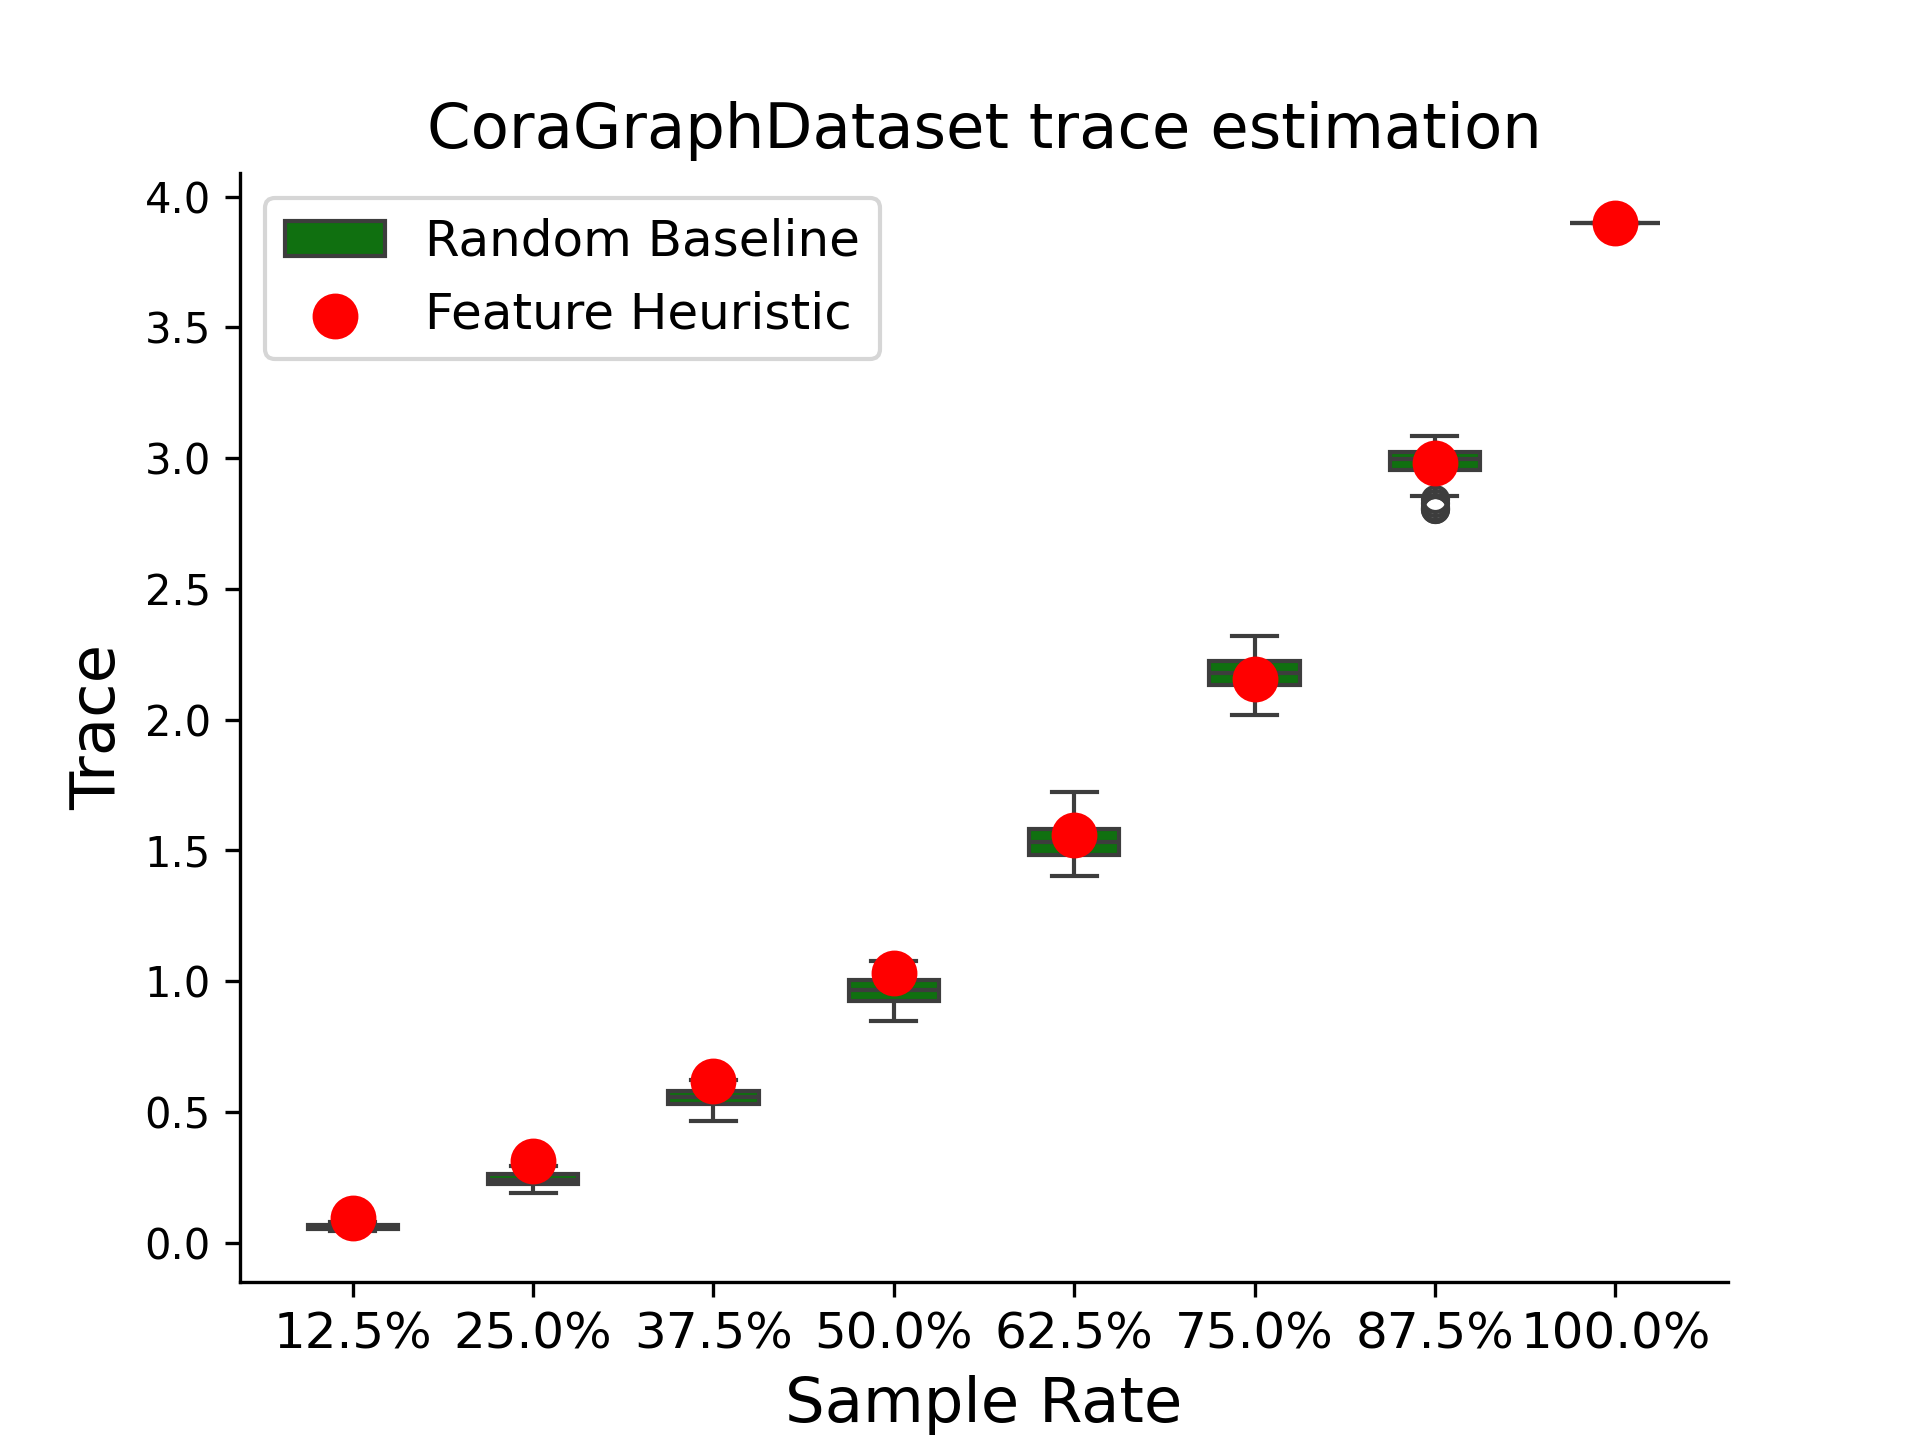
\includegraphics[width=0.32\textwidth]{img/trace_revised/CoraGraphDataset_trace_boxplot.png}
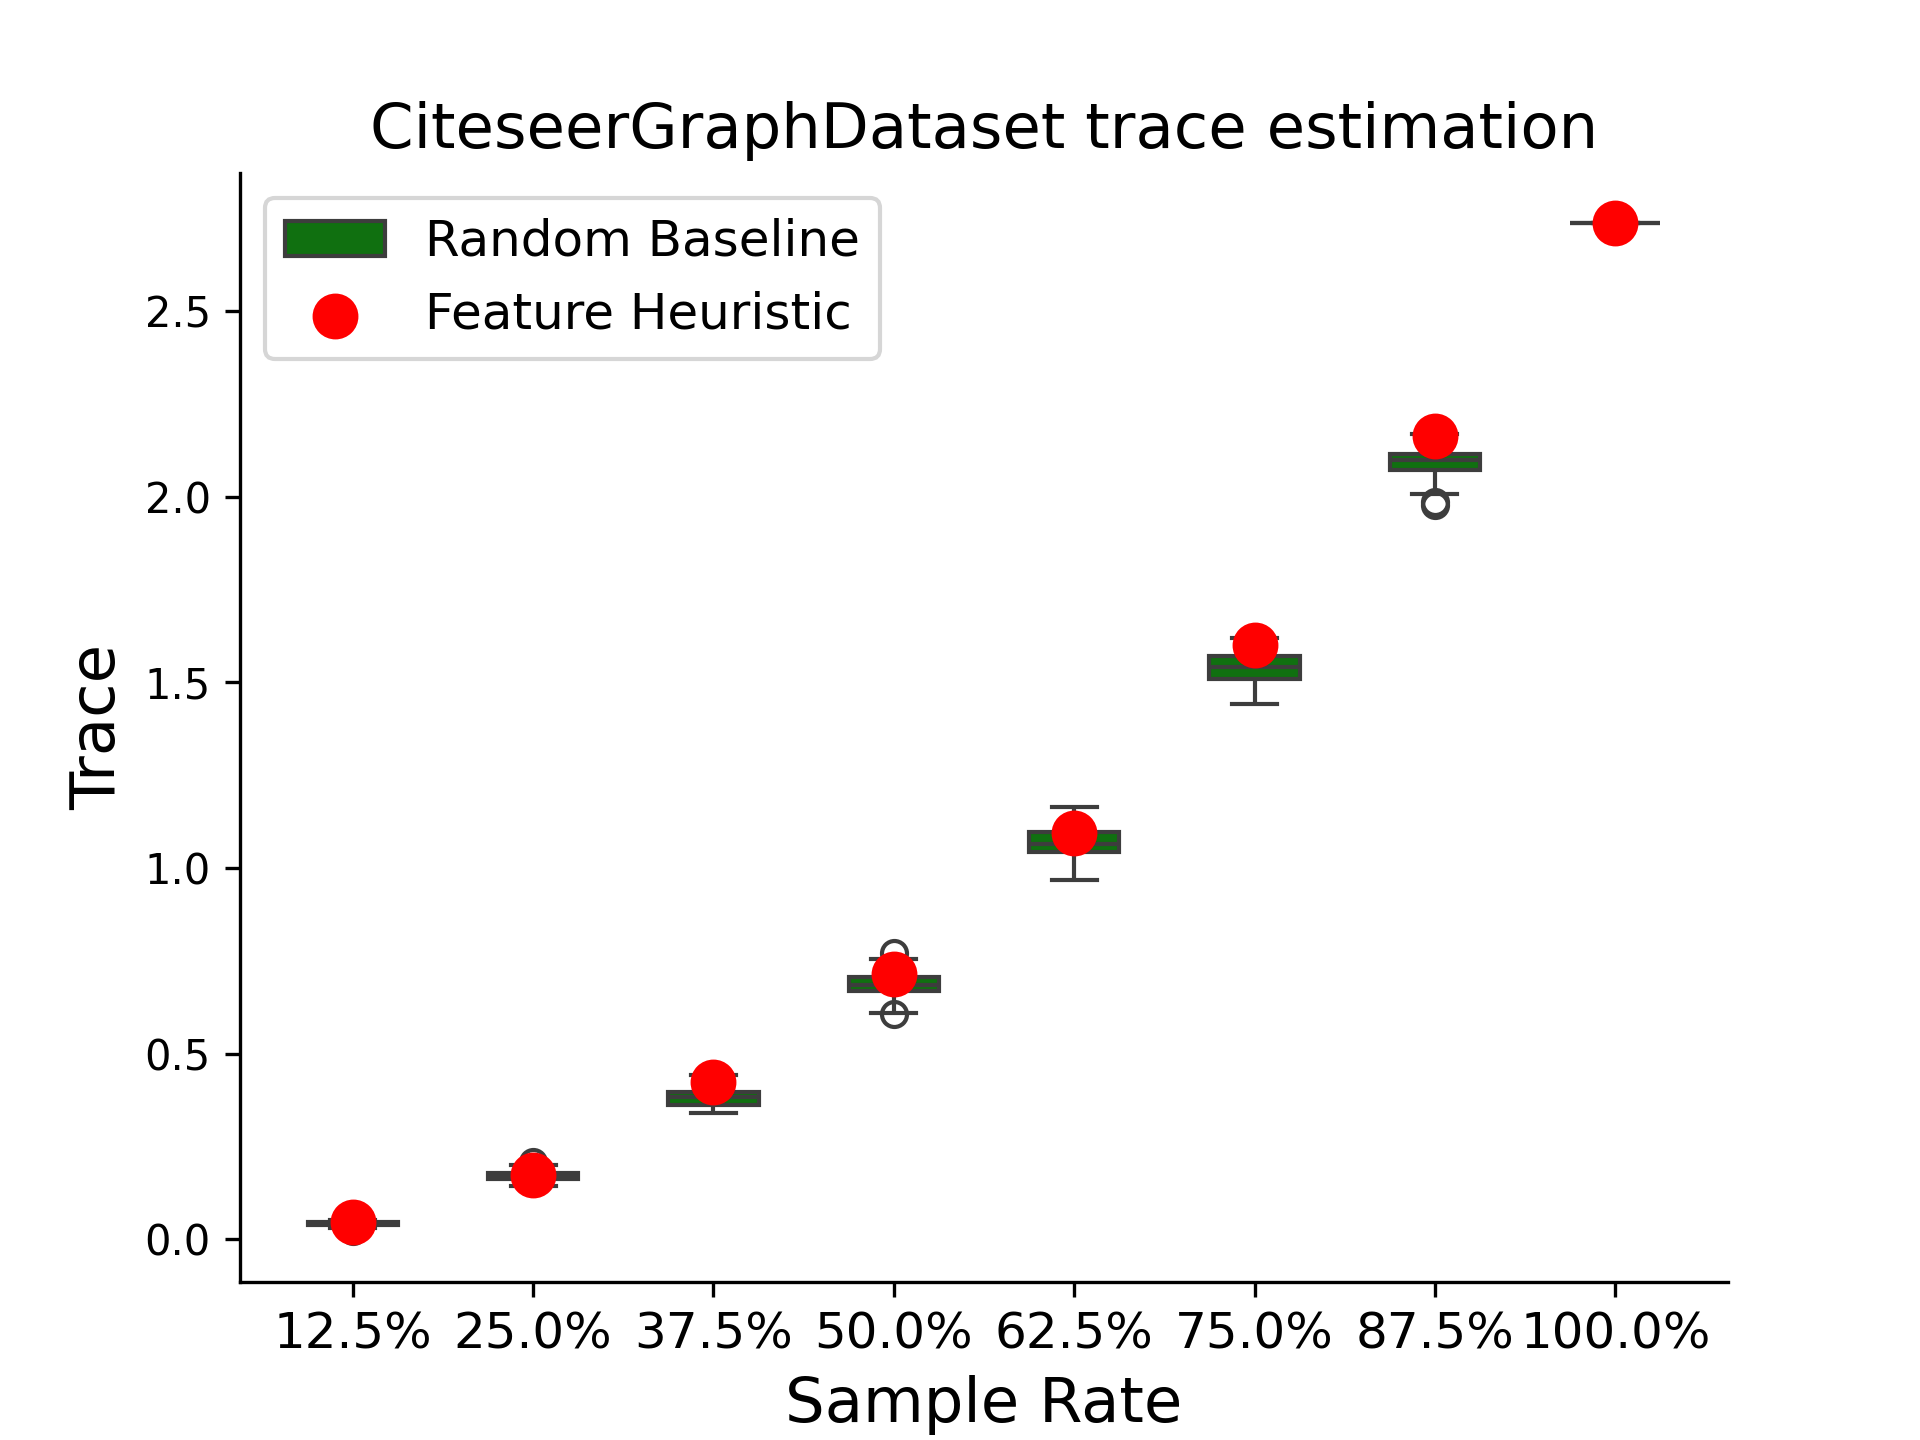
\includegraphics[width=0.32\textwidth]{img/trace_revised/CiteseerGraphDataset_trace_boxplot.png}
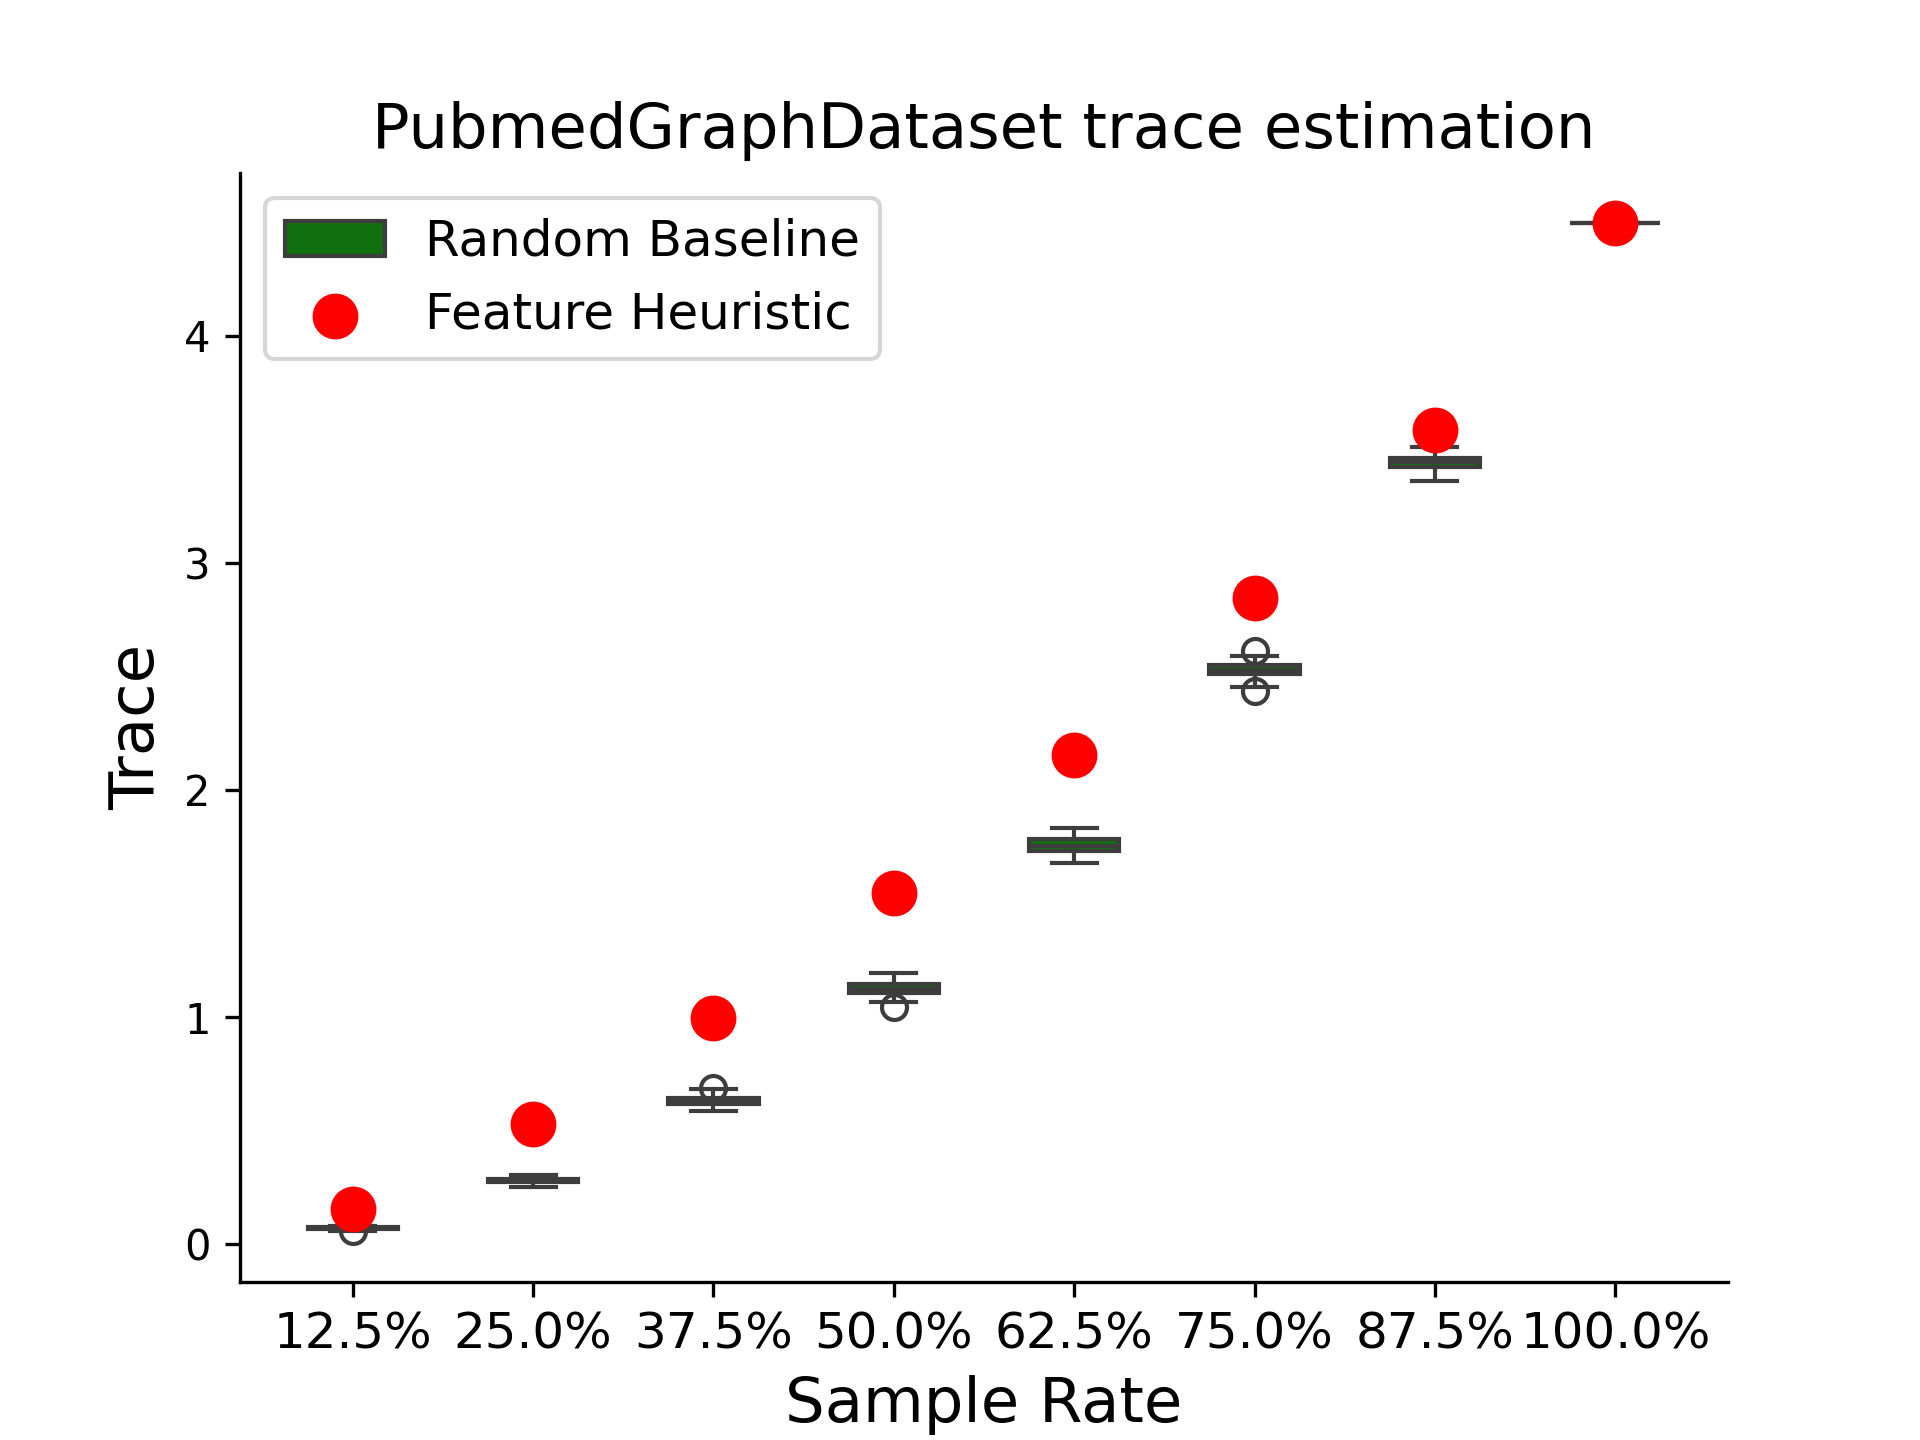
\includegraphics[width=0.32\textwidth]{img/trace_revised/PubmedGraphDataset_trace_boxplot.png}
\caption{This figure illustrates how does the trace of Laplacian change with respect to sample rate. Boxplots in the figure indicate the result obtained from random baselines in 50 runs, and the red dots are the adjusted trace of subgraphs generated by our sampling heuristic. Trace obtained by our result is almost always better than the average of random baselines except for Cora at 75\%. The adjusted trace is calculated by dividing the number of nodes in the subgraphs.}
\label{fig:trace}
\end{figure*}

\noindent \textbf{Expressivity.} While GNNs achieve remarkable performance in many graph machine learning tasks, they have fundamental limitations associated with their expressive power \cite{xu2018how,chen2019equivalence}. In GSP problems specifically, the expressivity of a GNN is constrained by the expressivity of the graph convolution, which in turn is constrained by the rank of the graph shift operator \cite{ruiz2024spectral}. This is demonstrated in the following proposition.

\begin{proposition}[Expressivity of Graph Convolution]
Let $G$ be an $n$-node symmetric graph with rank-$r$ graph shift operator $\mathbf{S}$, $r < n$, and $x \in \reals^n$ an arbitrary graph signal. Consider the graph convolution $\hat{y} = \sum_{k=0}^{K-1}h_k\mathbf{S}^kx$. Let $\ccalY \subset \reals^n$ be the subspace of signals that can be expressed as $y=\hat{y}$ for some $h_0, \ldots, h_{K-1}$. Then, $dim(\ccalY) \leq r + 1$.
\end{proposition}
\begin{proof}
   See the appendices of the extended version, available \red{\href{here}{here}}. 
\end{proof}

%\red{L: Check. James, can you check if the above proposition is true when you get a chance?}

In other words, the space of signals that can be represented with a graph convolution shrinks with the rank of the graph shift. Rank preservation is hence an important consideration when sampling subgraphs for training GNNs.



\begin{figure*}[t]
\centering
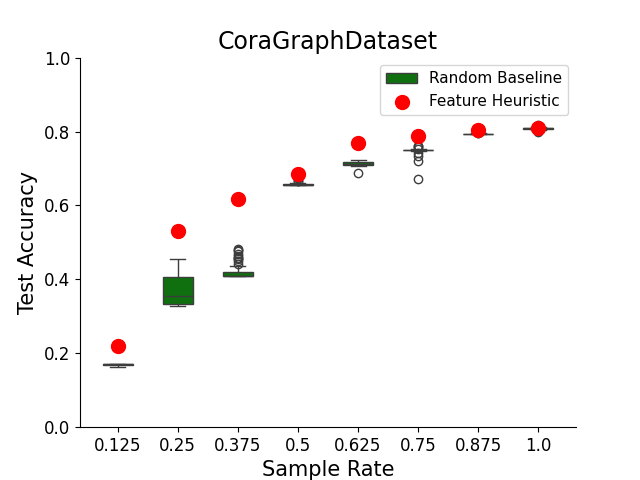
\includegraphics[width=0.32\textwidth]{img/GNN_acc_revised/CoraGraphDataset_undirected_random_baseline_boxplot.png}
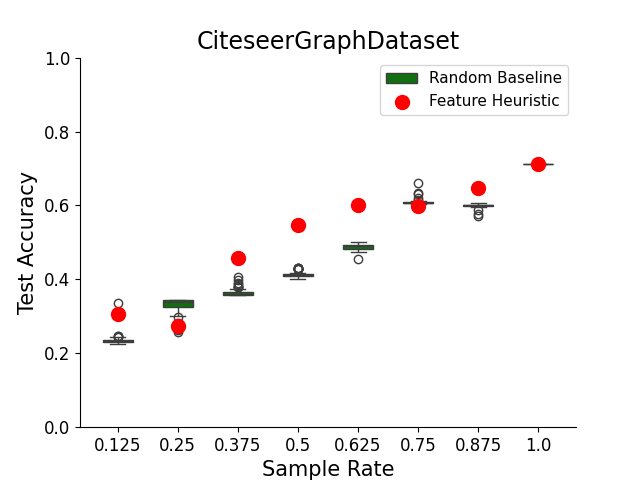
\includegraphics[width=0.32\textwidth]{img/GNN_acc_revised/CiteseerGraphDataset_undirected_random_baseline_boxplot.png}
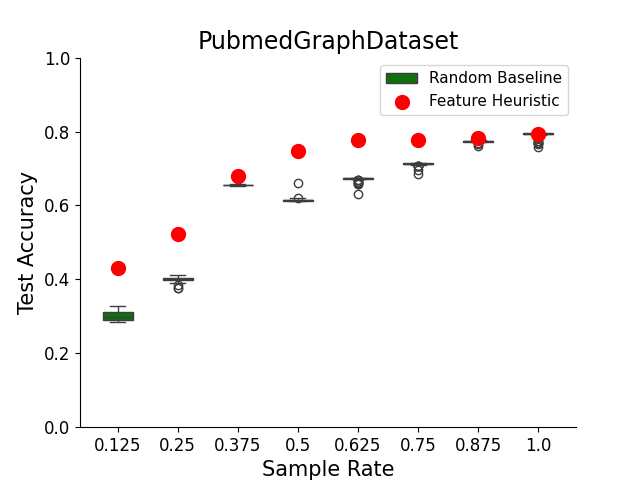
\includegraphics[width=0.32\textwidth]{img/GNN_acc_revised/PubmedGraphDataset_undirected_random_baseline_boxplot.png}
\caption{The red dots are the test accuracy of models tuned on each dataset at specific sample rates, with boxplots indicating the distribution of random baseline test accuracy. Our heuristic yields better results only except for Citeseer at 25\% of sample rate. Specifically, the differences of test accuracy are mostly recognizable at sample rates ranging from 37.5\% to 75\% across all three datasets. On average, accuracy grows slower as sample rate increases, intuitively because the marginal information is less significant with larger number of nodes already included in the subgraphs. }
\label{fig:GNN Acc}
\end{figure*}

\section{Feature homophily and homophily-based sampling}
%In this section, we present our theoretical contributions to the understanding of graph node downsampling. We firstly define feature homophily, then explain how it can be used to bound the trace of $\mathbf{L}$.

We start by introducing the notion of feature homophily, which is a requirement for our algorithm.
%and describe how graphs with moderate to high feature 
In order to make this definition compatible for graphs of different sizes, we first need to normalize $X \in \mathbb{R}^{n\times d}$ along both the feature and node dimensions. Explicitly, let $\Vec{\mu} = (\mu_1, \cdots, \mu_d)^T \in \mathbb{R}^d$ be the mean feature vector and $\Vec{\sigma} = (\frac{1}{\sigma_1}, \cdots, \frac{1}{\sigma_d})^T \in \mathbb{R}^d$ the standard deviation vector. We define the normalized graph features $\hat{X}$ as:
\begin{equation} \label{eqn:norm_features}
    \hat{X} = (X - \mathbf{1}_n \Vec{\mu}^T) \odot (\frac{1}{\sqrt{d}} \cdot \mathbf{1}_n \Vec{\sigma}^T) \text{.}
\end{equation}
%where $\mathbf{1}_n \in \mathbb{R}^d$ is a column vector of $n$ ones, and $\odot$ is Hadamard product. 
In other words, $\hat{X}[i,j] = \frac{X[i,j] - \mu_j}{\sqrt{d}\sigma_j}$. 
%Using the normalized feature matrix $\hat{X}$, we define a graph's feature homophily as follows.

\begin{definition}[Feature Homophily] \label{def:feature_homophily}
    Let $G$ be a graph with Laplacian matrix $\bbL$, and let $\hat{X}$ be the corresponding normalized feature matrix \eqref{eqn:norm_features}. The feature homophily of graph $G$ is defined as:
    \begin{equation} \label{eqn:feature_homophily}
        h_G = \frac{1}{n} \cdot \text{tr}(-\mathbf{L}\hat{X}\hat{X}^T)\text{.}
    \end{equation}
\end{definition}

%\textcolor{orange}{J: I revised the definition of feat homophily according to the weekly report. The previous typo couldn't match dimension in matrix multiplication. So it's not strictly a quadratic, but it's still non-positive but needs to be argued differently}

Since $\bbL$ is positive semidefinite and the trace of the outer product is the product of traces, it is ready to see, by Cauchy-Schwarz, that $h_G \leq 0$ for any undirected graph $G$. The larger the feature homophily $h_G$, i.e., the closer it is to $0$, the higher the alignment of the data $X$ (or, more precisely, of its principal components) with the low-frequency eigenvectors of $\bbL$---which account for most of the graph's global structure, such as its communities. Thus, the data is informative with regards to the graph. On the other hand, highly negative values of $h_G$ indicate strong alignment of $\hat{X}$ with high-frequency eigenvectors, which tend to be noisier and less descriptive of the graph structure.

%Just like how the typical homophily evaluates the alignment of labels between the nodes and their neighbors, feature homophily examines the alignment of features. The reason why we used $\mathbf{L}$ to substitute $\mathbf{A}$, which is used in the definition of edge/typical homophily, is that the Laplacian has the desired property of being a positive semi-definite matrix while preserving the connectivity information. 

%And with the help of Cauchy-Schwartz inequalities on Frobinius inner product, we have the following inequality holds.

The following proposition provides a lower bound on the trace of the graph Laplacian in terms of the feature homophily $h_G$.

\begin{proposition}[Lower Bound on $\text{tr}(\bbL)$]
    \label{bound on tr L}
    \begin{equation} \label{eqn:bound_tr_L}
        \text{tr}(\bbL)^2 \geq - \frac{h_G}{\text{tr}(\hat{X}\hat{X}^T)^2}
    \end{equation}
\end{proposition}
%\textcolor{orange}{J:It looks wired if I put the proof of proposition 3.3 inside the proof of 3.2 because there's no clear division between the statement and the proof of 3.3.w}
\begin{proof}
See the appendices of the extended version, available \red{\href{here}{here}}.
\end{proof}

Note that if the graph $G$ has high feature homophily, the right-hand side of \eqref{eqn:bound_tr_L} is small, and thus the lower bound on $tr(\bbL)$ is approximately vacuous. Conversely, for heterophilic graphs, $h_G$ has higher magnitude, so the lower bound is further away from zero.

\noindent \textbf{Algorithm.} Although simple, the result from Proposition \ref{bound on tr L} has important implications for feature-homophilic graph sampling. Suppose we start removing nodes from $G$ according to the diagonal entries of $X X^T$  sorted in decreasing order, so that the denominator on the right-hand side of \eqref{eqn:bound_tr_L} becomes progressively smaller. If $G$ is homophilic with $h_G \approx 0$, the decrease in the denominator $tr(\hat{X}\hat{X}^T)$ is likely to lead to an increase of the lower bound on $tr(\bbL)$. Therefore, we obtain lower bounds on $tr(\bbL)$ that are increasingly more meaningful and, as a result, that ensure rank preservation in the sampled graph. This idea is formalized in Algorithm \ref{alg:sampling}.

\begin{algorithm}[t]
\caption{Node Sampling for Feature-Homophilic Graphs}
\begin{algorithmic}
    \Require $G(V, E)$, $|V|=n$; $X \in \reals^{n \times d}$; $\gamma \in [0,1]$
    \vspace{2pt}
    \State Calculate deletion budget: $n_d \gets \lfloor (1 - \gamma) \cdot n \rfloor$
    \State Calculate node scores: $\Vec{s} \gets \text{diag}(XX^T)$
    \State Keep $n-n_d$ nodes with  highest score:
    
    $\text{idx} \gets \text{argmax}(\Vec{s}, \;\text{descending}=\text{True})[n_d:n]$
    \State Sample graph:
    
    $\tilde{V} \gets V \cap \text{idx}$
    
    $\tilde{E} \gets \{(u,v): u,v \in \tilde{V}, (u,v) \in E \}$
    
    $\tilde{X} \gets X[\text{idx},:]$
    \vspace{2pt}
    \State \Return $\tilde{G}(\tilde{V}, \tilde{E})$; $\tilde{X}$
\end{algorithmic}
\label{alg:sampling}
\end{algorithm}

\noindent \textbf{Complexity.} When $d<n$, as is often the case in practice, Algorithm \ref{alg:sampling} offers lower computational complexity than graph sampling algorithms with rank preservation objectives, as demonstrated by Proposition \ref{prop:complexity}.

\begin{proposition}[Complexity of Algorithm 1] \label{prop:complexity}
    Let $G=(V,E)$ be a graph with $|V|=n$ and $|E|=m$, and let $X \in \reals^{n\times d}$ be the corresponding node feature matrix. For any sampling budget $\gamma$, the complexity of Algorithm \ref{alg:sampling}, including computation of $h_G$, is $O(dm)$. If $G$ is known to be feature-homophilic, computation of $h_G$ can be bypassed and the complexity simplifies to $O(dn)$. 
\end{proposition}
\begin{proof}
See the appendices of the extended version, available \red{\href{here}{here}}.
\end{proof}

Importantly, the complexity of Algorithm \ref{alg:sampling} is dominated by the complexity of calculating the feature-homophily, which only has to happen once prior to execution to determine if the graph is homophilic. The complexity is further independent of the sampling budget, as the diagonal elements of $XX^T$ only have to be computed and sorted once. 

On sparse graphs ($m \ll n^2)$ with moderate feature dimension $d$, Algorithm \ref{alg:sampling} is cheaper than direct maximization of $tr(\bbL)$, which requires $O((1-\gamma)n^2)$ computations---$O(n)$ node degree computations $(1-\gamma)n$ times, as node degrees change each time a node is removed from $G$. In fact, this is an underestimation, as it does not factor in the cost of breaking ties across nodes with the same degree. Algorithm \ref{alg:sampling} is also notably cheaper than spectral algorithms such as \cite{chen2015discrete, anis2016efficient} which are inspired by E-optimal sampling and, without exhaustive search, require greedy routines with complexity at least $O(\gamma nm)$. Another advantage of Algorithm \ref{alg:sampling} is that it does not require sequential execution, unlike maximization of $tr(\bbL)$ and \cite{chen2015discrete,anis2016efficient}, which cannot be parallelized.

%\red{L: Upon further consideration, I think we shouldn't discuss the three scenarios. It's too informal.}
\section{Experimental Results}

In this section, we present a further analysis on our sampling algorithm. Also, by comparing the test accuracy between models trained on subgraphs sampled by our algorithm and random baselines, we conclude the effectiveness and robustness of our proposed method. 

% To execute this algorithm, we need a graph and a sample rate $\gamma$ as input. We firstly denote $N$ as the number of nodes to exclude, and then calculate feature score $S$ as the diagonal of $XX^TXX^T$. After that, we obtain the sorted index of $S$ and our subgraph $\tilde{G}$ accordingly, over which we will be training with better efficiency. 

\noindent \textbf{Trace preservation.} Among many ways to evaluate a sampling algorithm over a graph, apart from test accuracy benchmarks which we will show in Figure \ref{fig:GNN Acc}, one of the most frequently used, and probably most informative one is the rank of $\mathbf{L}$. However, because the estimation on the rank of $\mathbf{L}$ is almost infeasible due to the high dimensionality, trace is often used as a mediate. With the lower bound we proposed in Proposition \ref{bound on tr L}, empirically from Figure \ref{fig:trace} we see that across all three datasets, our sampling method results in subgraphs with larger adjusted $\tilde{\text{tr}}(\textbf{L}) = \text{tr}(\mathbf{L}) / n$  at almost all sample rates compared with the average of random baselines. This pattern is especially obvious over PubMed dataset.

\noindent \textbf{GNN training.} As for GNN experiments, for each dataset at a given sample rate, we firstly tune the best configuration for our sampling algorithm as shown in the following, then test the same configuration on random baselines with 50 different runs. Specifically, the valid/test accuracy obtained in the training and evaluation process is based on original full-size graph, which means we only limit the training process to the sampled subgraphs. This pipeline is ideal because it simulates the process of training and model selection, which makes the experiments more indicative for general purposes. 

\noindent \textbf{Experiment details.} For each dataset and sample rate, we chose hidden dimension in $\{64, 128\}$, number of layers in $\{1,2,3\}$, number of epochs in $\{200, 300\}$, learning rate and weight decay in $\{0.001, 0.0001\}$, GCN model type in $\{\text{GCN}, \text{SAGE}\}$ with all ReLU activation between all layers, and used Adam as our optimizer. All of the graphs are configured to be undirected by adding edges of the opposite direction before being fed into the networks. 

It is worth mentioning that the GNN of our choice is rather simple. This is because the power of a sampling method can be more apparent and easier to identify if model complexity is relatively restrained. In Figure \ref{fig:GNN Acc}, where the box plots represent the distribution of random baseline accuracy, the test accuracy acquired by our model(the red dots) are all better by a distinctive margin except for Citeseer at sample rate 25\%. In other cases, for instance, all three datasets at a sample rate of 62.5\%, our heuristic won by around 10\% of accuracy.
\section{Conclusions}

In this paper, we introduced a novel graph sampling algorithm that leverages feature homophily to efficiently preserve the structural properties of large graphs. 
%By minimizing the trace of the feature correlation matrix, our method preserves the graph rank, which is crucial for maintaining GNN expressivity in homophilic graphs. With its lower computational complexity compared to spectral methods, our algorithm offers a more practical solution for GNN training on large-scale networks. 
Compared with random sampling, our proposed sampling heuristic is not only more effective in preserving the trace/rank of the graph, but also achieves superior performance when it is used to sample graphs for GNNs trained via transferability. These empirical results indicate the strong potential of our heuristic. Future work will focus on larger graph datasets such as ogbn-mag, where efficient training on subgraphs is even more pressing.
%Experimental results on citation networks demonstrate that our approach outperforms random sampling in both trace preservation and transferability performance. Future work may explore extending this method to other graph types and further refining its theoretical guarantees.




\vfill\pagebreak

% References should be produced using the bibtex program from suitable
% BiBTeX files (here: strings, refs, manuals). The IEEEbib.bst bibliography
% style file from IEEE produces unsorted bibliography list.
% -------------------------------------------------------------------------
\bibliographystyle{IEEEbib}
\bibliography{myIEEEabrv,strings,refs,bib_cumulative}

\appendix 
\begin{proof}[Proof of Prop. II.2]
  From the definition, we can rewrite 
    $$\ccalY = \text{span}(\{S^kx : k=0, \ldots, K\})$$
    Since $\mathbf{S}$ is symmetric, there exists some $\mathbf{E}, \mathbf{\Sigma} \in \mathbb{R}^{n \times n}$ satisfying $\mathbf{E}\mathbf{E}^T = \mathbf{I}_n$ and $\mathbf{\Sigma}$ diagonal, such that $\mathbf{S} = \mathbf{E}\mathbf{\Sigma}\mathbf{E}^T$. This implies a simple explicit representation for $\mathbf{S}^k = \mathbf{E}\mathbf{\Sigma}^k\mathbf{E}^T$. As a result, $\mathbf{S}^k$ share not only the same rank, also the same coordinates regardless scaling. So for any given $x\in \reals^n$, rank($\{S^kx : k=1, \ldots, K\}$) $\leq$ rank$(\mathbf{S}) = r$. Therefore, we have $dim(\ccalY) \leq r+1$ with $x$ as an additional coordinate candidate.
\end{proof}

\begin{proof}[Proof of Prop. III.2]
By the definition of feature homophily, and using the Cauchy-Schwarz inequality, we write
\begin{equation}
    -h_{G} = tr(\bbL XX^T) = \langle \bbL, XX^T \rangle_F \leq \| \bbL \|_F^2 \cdot \|XX^T\|_F^2 \text{.}
\end{equation}

Now we rewrite it in terms of trace
\begin{equation}
    \| \bbL \|_F^2 \cdot \|XX^T\|_F^2 = tr(\bbL^2) tr((XX^T)^2) \text{.}
\end{equation}

Because both $\bbL^2$ and $(XX^T)^2$ are positive semi-definite, we have
\begin{equation}
    tr(\bbL^2) tr((XX^T)^2) \leq tr(\bbL)^2tr(XX^T)^2 \text{.}
\end{equation}

Finally, combining the above equations, we get the desired result
    \begin{equation}
        -h_G \leq \text{tr}(\bbL^2)\text{tr}((\hat{X}\hat{X}^T)^2) \leq \text{tr}(\bbL)^2\text{tr}(\hat{X}\hat{X}^T)^2 \text{.}
    \end{equation}
\end{proof}

\begin{proof}[Proof of Prop. III.3]
Algorithm \ref{alg:sampling} involves two main steps: computation of the homophily $tr(-\bbL XX^t)$, and of the node scores $\mbox{diag}(XX^T)$. Computation of $tr(-\bbL XX^t)$ has complexity $O(dm)$, as it is dominated by computing the matrix-matrix multiplication $\bbL X$ and the subsequent trace computation only requires $O(dn)$. Similarly, the computation of $\mbox{diag}(XX^T)$ requires $O(dn)$ as we only calculate the diagonal elements of $XX^T$.
\end{proof}

\end{document}
